\subsection{Osciladores amortiguados}

  \PN En muchos sistemas reales, fuerzas no conservativas como la fricción o la resistencia del aire retardan el
  movimiento del sistema. En consecuencia, la energía mecánica del sistema disminuye en el tiempo y se dice que el
  movimiento está amortiguado.

  \vspace{3mm}
  \PN Consideremos el siguiente modelo:

  \begin{figure}[H]
  \centering
    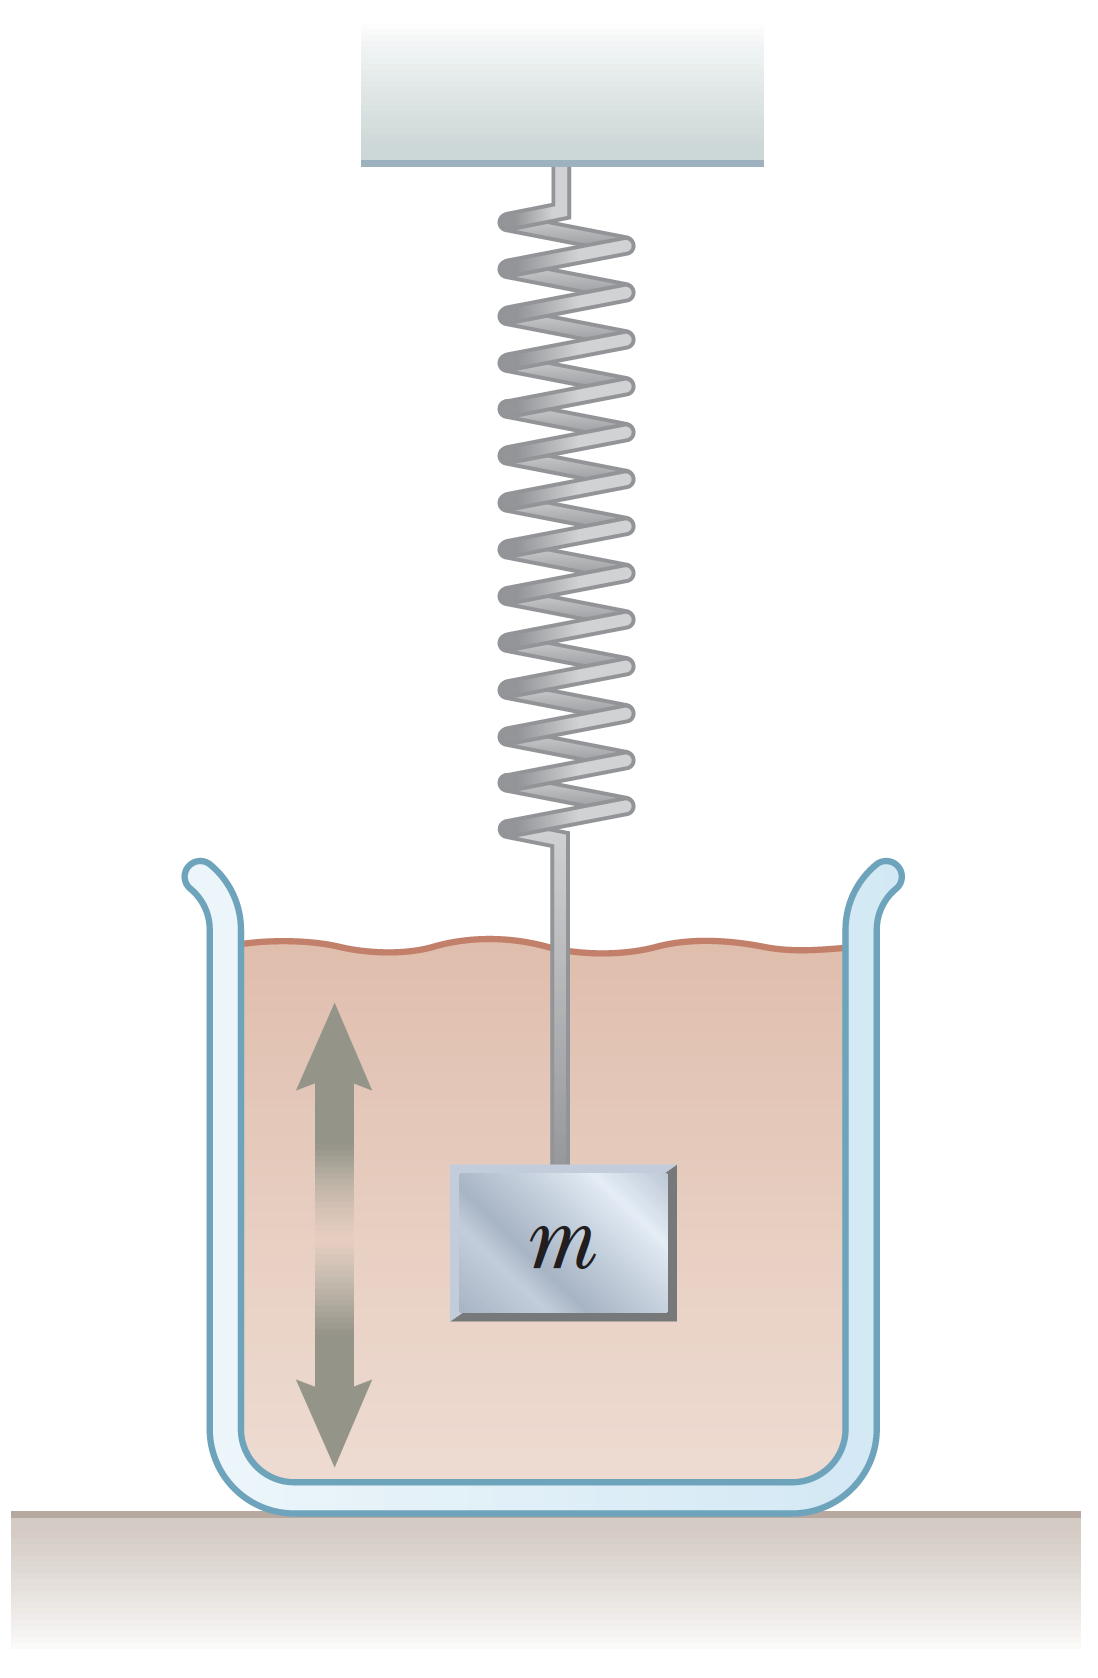
\includegraphics[width=0.15\textwidth]{2/figure_2}
    \caption{Ejemplo de un oscilador amortiguado es un objeto unido a un resorte y sumergido en un líquido viscoso.}
  \end{figure}

  \PN Se puede escribir la segunda ley de Newton como:
  \begin{eqnarray*}
    \Sigma \ F_{x} &=& -kx - \underbrace{b \overbrace{v}^{\text{coeficiente de amortiguamiento}}}_{\text{fuerza retardadora}} = ma_{x} \\
    -kx - b \frac{dx}{dt} &=& m \frac{d^{2}x}{dt^{2}}
  \end{eqnarray*}

  \PN \textbf{Ecuación de la posición}
  \begin{equation}
    x(t) = A \mathrm{e}^{\frac{-b}{2m}t} \cos (\omega t)
  \end{equation}

  \PN donde la frecuencia angular de oscilación es:
  \begin{equation}
    \omega = \sqrt{\frac{k}{m} - \left(\frac{b}{2m}\right)^{2}}
  \end{equation}

  \PN Es conveniente expresar la frecuencia angular de un oscilador amortiguado en la forma:
  \begin{equation}
    \omega = \sqrt{\omega_{0} - \left(\frac{b}{2m}\right)^{2}}
  \end{equation}

  \PN donde $\omega_{0} = \sqrt{k/m}$ representa la frecuencia angular en ausencia de una fuerza retardadora (el
  oscilador no amortiguado) y se llama \textbf{frecuencia natural} del sistema.

  \pagebreak
  \PN \textbf{Tipos de amortiguamiento}
  \begin{itemize}
    \item Subamortiguado: $\omega_{0} > \frac{b}{2m}$
    \item Críticamente Amortiguado: $\omega_{0} = \frac{b}{2m}$
    \item Sobreamortiguado: $\omega_{0} < \frac{b}{2m}$
  \end{itemize}
